\documentclass[12pt]{article}

\usepackage[UTF8]{ctex}
\usepackage{appendix}
\usepackage{enumerate}
\usepackage{amsmath}
\usepackage{graphicx}
\usepackage{cite}
\usepackage{bigstrut}
\usepackage{geometry}
\geometry{left =2.5 cm,right=2.5cm,top=2.5cm,bottom=2.5cm}
\usepackage{multirow}
\usepackage{lastpage}
\usepackage{longtable}
\usepackage{listings}
\usepackage[section]{placeins}
\usepackage[colorlinks,linkcolor=blue]{hyperref}
\date{}
\geometry{a4paper,scale=0.8}
\title{\zihao{2}\textbf{作品说明书}}
\author{\zihao{3}\textbf{基于51单片机的带声光提示的多功能计分抢答器}}
\date{\zihao{3}2019.3}
\begin{document}%文档从这里开始。

\numberwithin{footnote}{section}
\renewcommand{\contentsname}{\centering 目录}
\renewcommand{\tablename}{表}
\renewcommand{\figurename}{图}
\renewcommand\refname{参考文献}
\renewcommand\appendix{\setcounter{secnumdepth}{0}}
\renewcommand\abstractname{摘要}

\maketitle
\zihao{4}
\section{产品背景}
随着各种知识竞赛和文娱活动的兴起,单凭人工操作的的抢答判断会因为主持人的误判而逐渐受到挑战,使比赛丧失公平性。各类抢答器响应需求纷纷上市,市面上的现有抢答器大多仅具有抢答的功能,比较单一;有些兼具计分功能的产品又无法灵活的改变分值大小,只能规定好特定分数,无法灵活根据题型进行改变;有线抢答器装置较为繁琐,说明书冗长;较高端的无线抢答器,尤其是一些具有较为完备的功能的,价格则十分昂贵,动辄达到千元以上,不能满足对经费有限制的,活动规模不大的抢答比赛的需求。同时,倘若对于电路的设计和程序进行修改和扩展,还能够进行大规模投票,抽奖,报警等附加功能,可适用于不仅仅是抢答比赛这一单一情境,应用前景良好。

据此,我们的产品除了基础的抢答倒计时、违规抢答报警及计分功能外,还具备了如下拓展功能:
\begin{enumerate}
  \item 能够人工设置抢答限时、答题限时时长及各类分值大小;
  \item 在一轮抢答结束后,显示选手抢答时间,增强比赛公平性;
  \item 使用LCD屏幕显示得分并进行当前分数排序;
  \item 使用无线按键,并可使用按键灯光颜色显示选手抢答的正确与否。
\end{enumerate}

该作品基于51单片机的控制系统,功能齐全,易于操作,响应时间短,计时准确,相较市面上的众多抢答器实用性更强。

\section{系统结构}
该系统的系统框图及软件程序流程图分别见图\ref{fig:kuangtu}及图\ref{fig:kuangtu2}。
\begin{figure}[h]
	\centering
	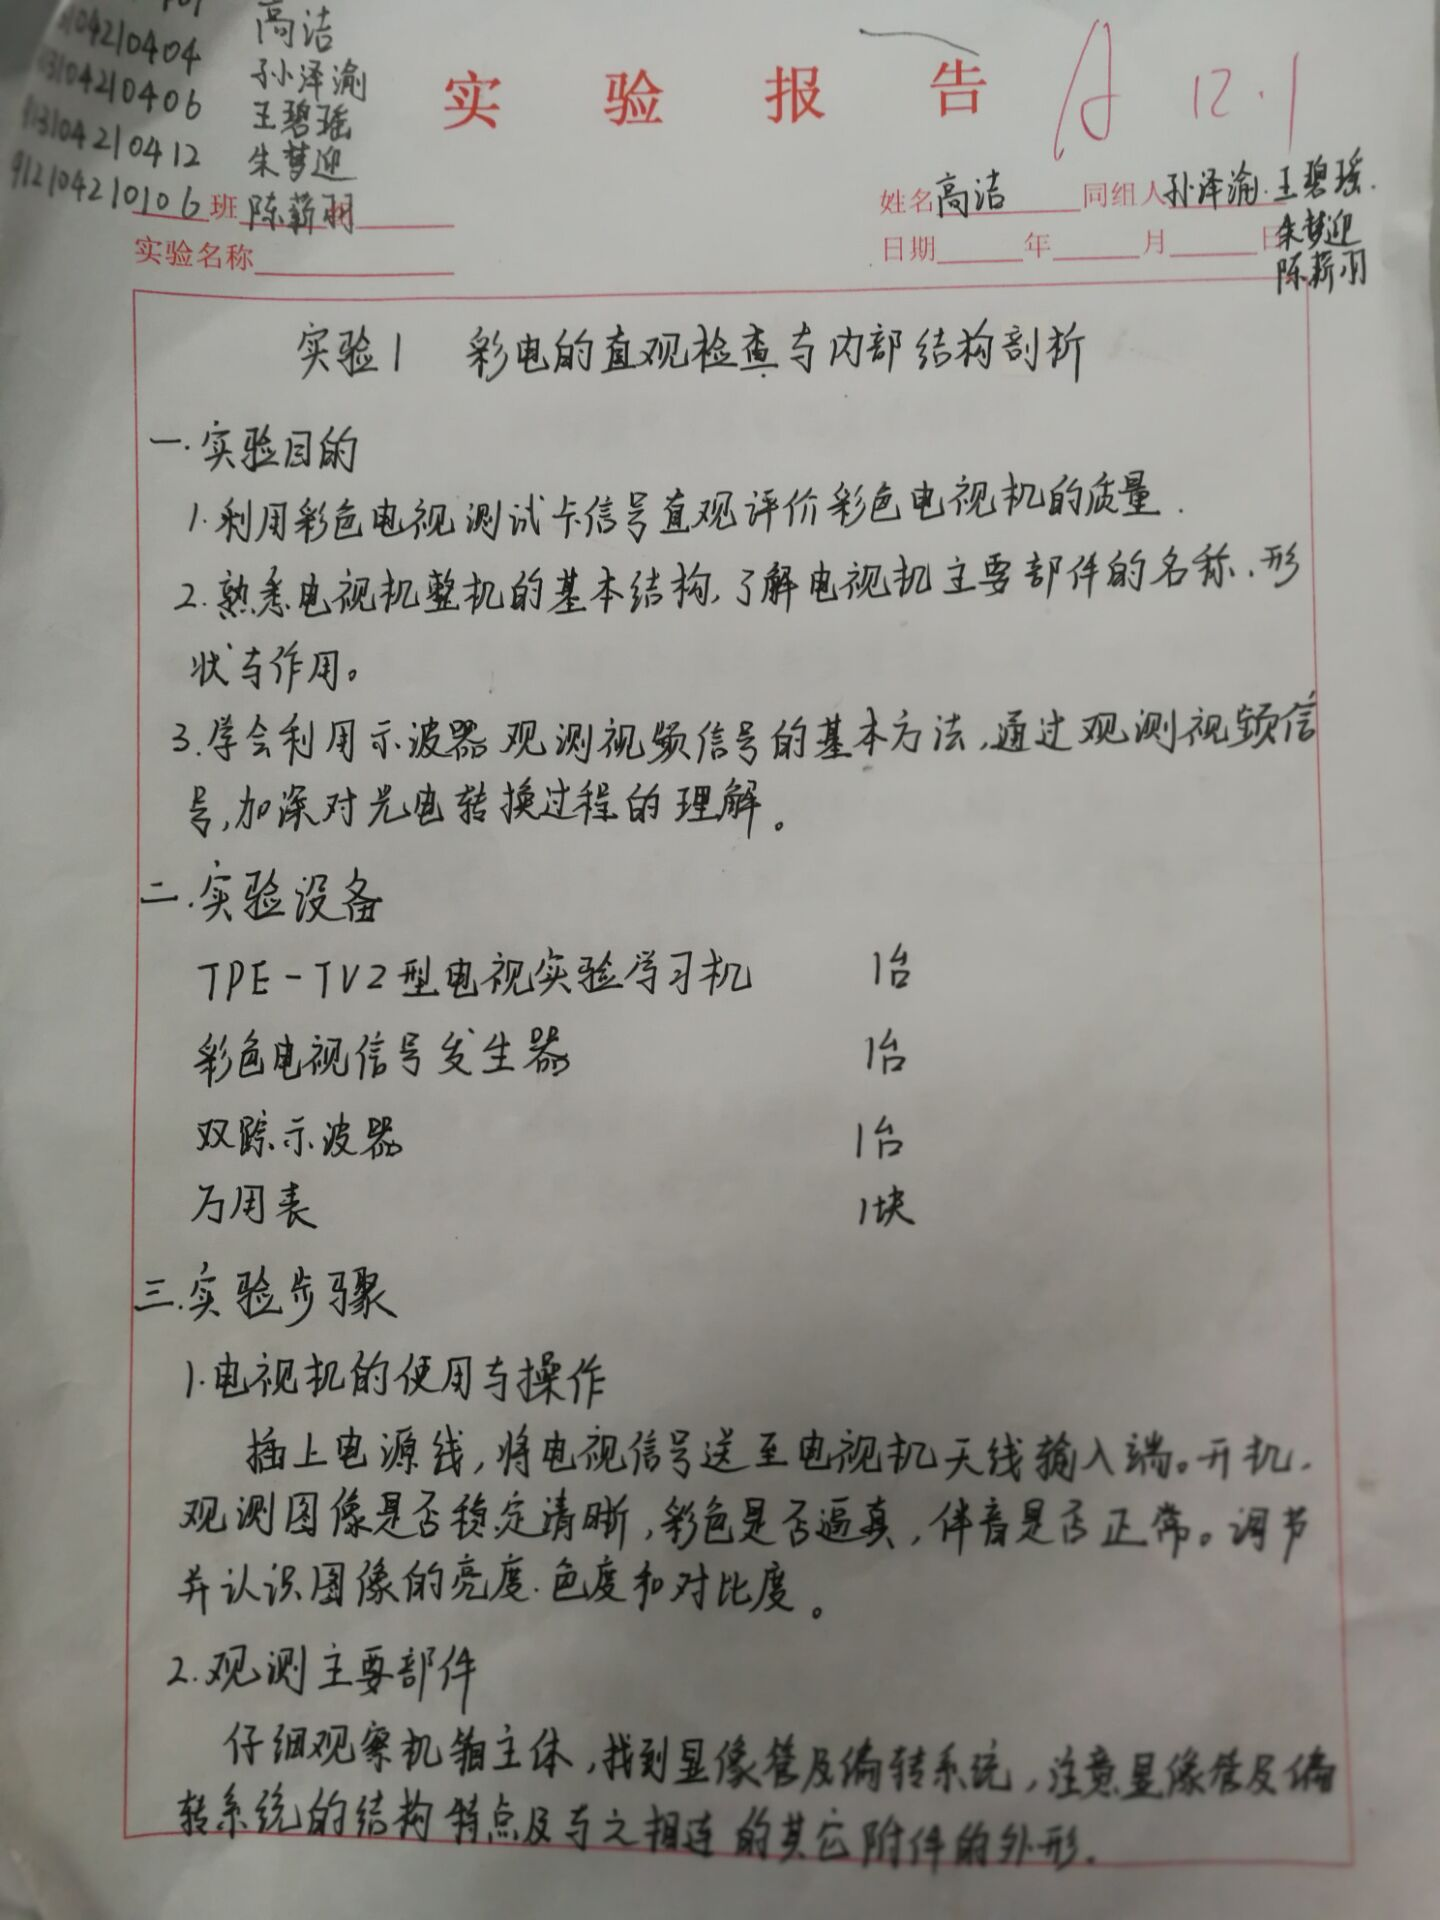
\includegraphics[width=0.8\linewidth]{picture/01.jpg}
	\caption{系统框图}
	\label{fig:kuangtu}
\end{figure}

\begin{figure}[h]
	\centering
	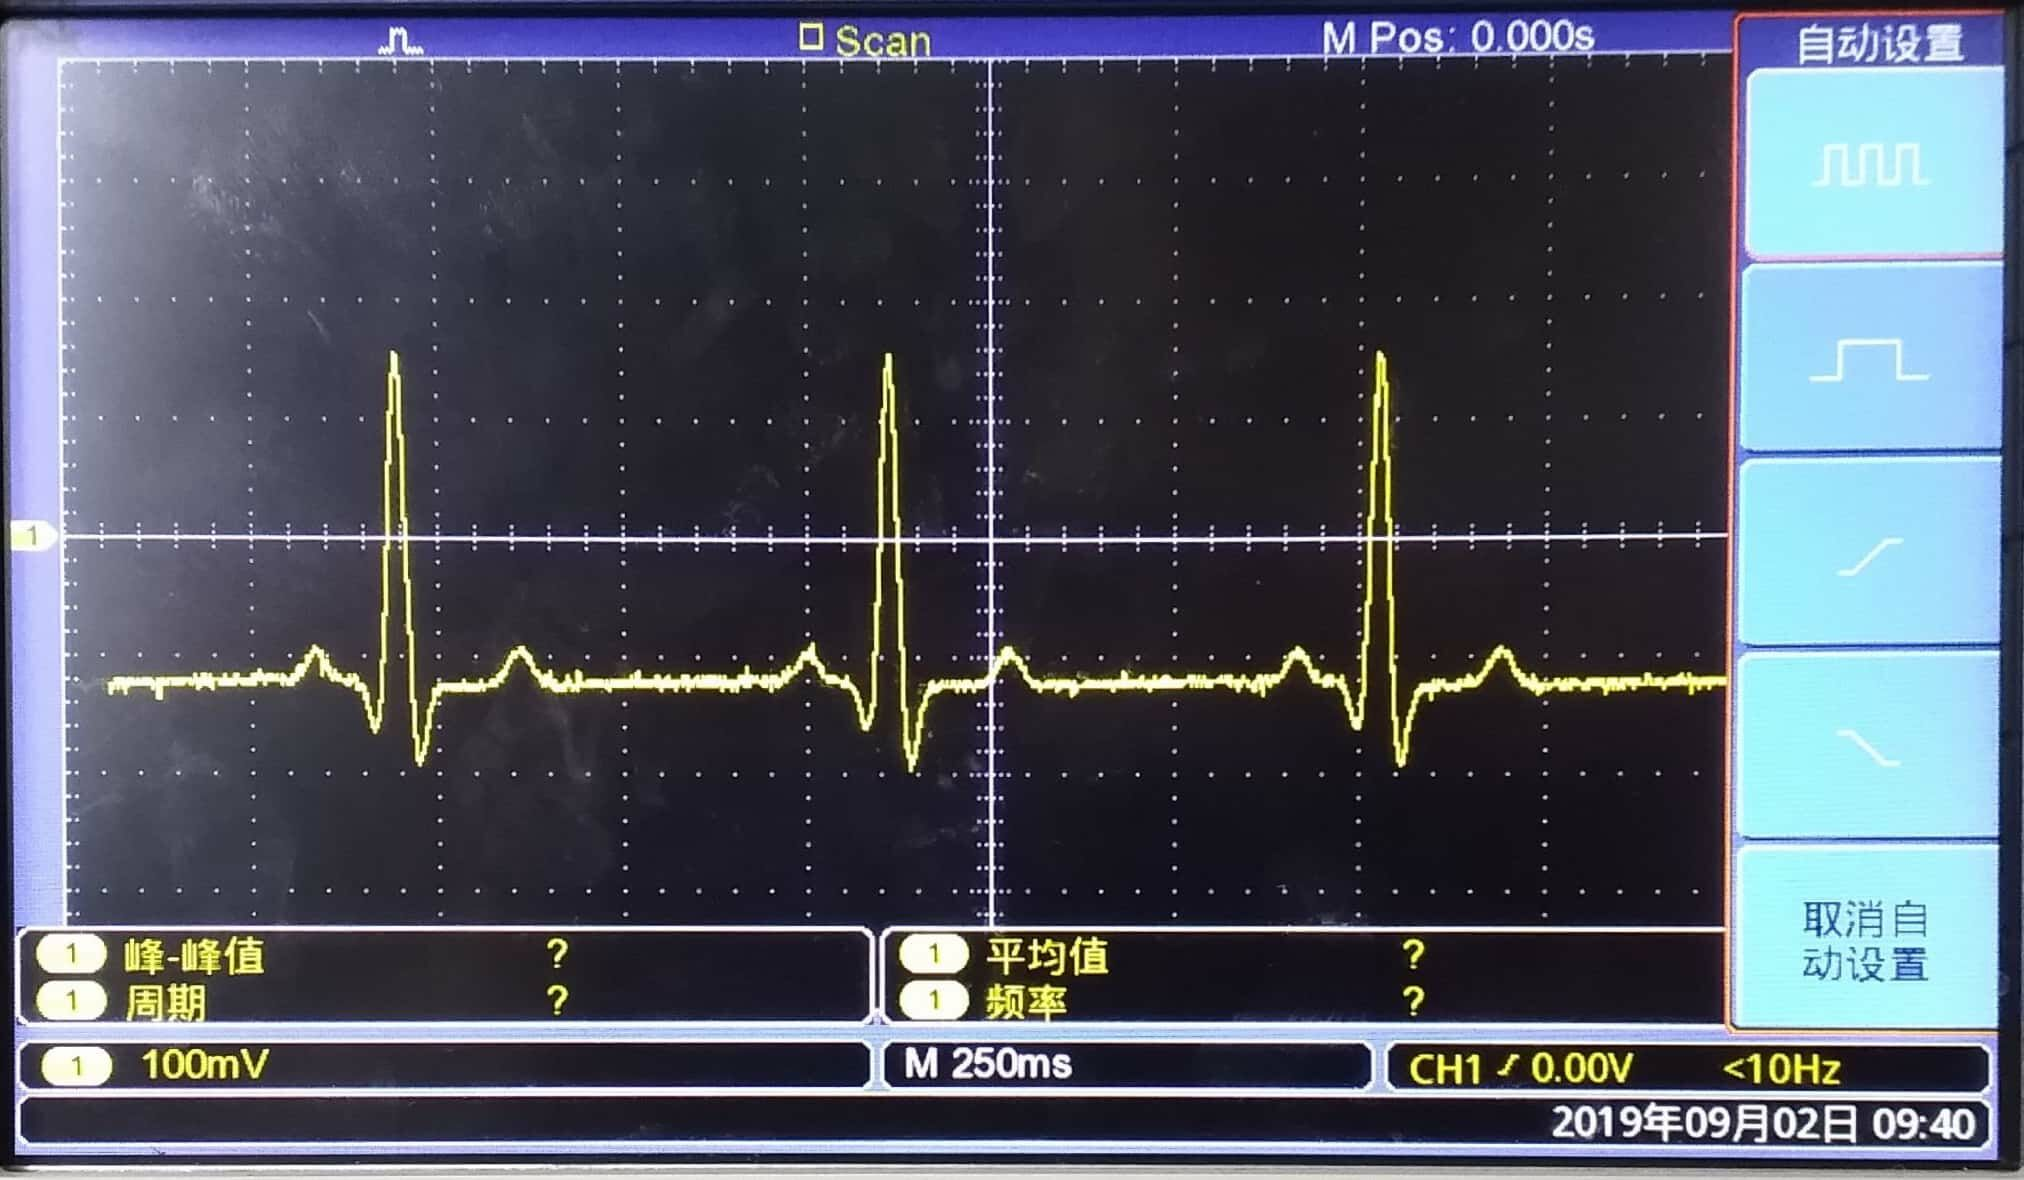
\includegraphics[width=0.7\linewidth]{picture/02.jpg}
	\caption{软件程序流程图}
	\label{fig:kuangtu2}
\end{figure}
\section{主要功能}
该抢答器的具体功能如下:
\begin{enumerate}
  \item 此智力竞赛抢答器设置了8个按键,可同时供8名选手或8名代表队参加比赛,每队设置一个抢答成功提示led灯,蜂鸣器,8队选手公共用块计分显示屏。
  \item 主持人需操作4个控制开关,可切换5项功能模式。
  \begin{enumerate}[模式1:]
    \item 基本倒计时抢答模式,主持人按下开始按钮后,选手开始抢答,若有人违规则蜂鸣器报警,并显示违规选手号码并扣分。抢答结束后,可显示选手抢答时间。
   \item  答题时间倒计时模式,主持人按下开始按钮后,选手开始作答,并且由主持人人工判断答题的正误为选手加分减分;
\item 在LCD显示屏上查看选手得分及当前分数排名;
\item 设置抢答时间和答题时间;
\item 设置违规扣分值、答题正确加分值、答题错误扣分值。
  \end{enumerate}
  \item 开始抢答后,主持人手动按下控制键开始倒计时,若发生意外情况可暂停倒计时; 同时,8名选手开始抢答,若有人违规,则在屏幕上显示号码并进行蜂鸣器报警;若无人抢答,则倒计时至结束并且显示“Time out”并进行报警。若有选手抢答成功,则显示其号码并进行蜂鸣器提示。此题抢答结束后可查看各位选手的抢答时间。随后,由主持人判断开始答题倒计时。若答题正确,则由主持人按键进行加分。在答题结束后,切换至模式三,可显示八人的比赛得分;若需要调节抢答和答题倒计时,则可使用模式四进行调节;若需要调节分值,则可使用模式五进行调节。
\end{enumerate}

本产品在前一次参赛的基础上又增加了一些改良,首先,使用更大的led屏幕方便选手查看自己的得分;其次,更改了按钮的类型,使得抢答过程更为顺手和方便;最后,为了防止因无法判断到底是谁先进行抢答而争吵的状况,本产品新增了计时电路记录每个人的抢答时间,并且显示在led屏幕上,可以很好地判断到底是谁完成了抢答。除此以外,还增加了无线按钮,使得选手不必聚集于单一的抢答器周围,可以自由选择答题位置。并且,可以根据选手面前的led灯闪烁状况判断答题是否正确。

本文设计的抢答器以51单片机为核心,采用组合逻辑电路和时序逻辑电路相结合的设计思路,完成数字抢答器的设计。它在日常各种智力竞赛中被广泛应用。为丰富人们日常生活的各种智力竞赛提供方便,具有良好的应用前景。

\section{产品优势与创新性}
市面上现有抢答器普遍存在精确度低、功能单一等问题,为满足各种知识竞赛和文娱活动的需求,对此类缺陷做出改进,本次作品设计了一款性能更加优越的多功能抢答器。
\begin{enumerate}
  \item \textbf{较市面上大多数抢答器功能更加齐全}

该产品与以往市面上的抢答器相比,功能更加齐全,包含有违规报警、抢答计时、答题计时、选手分数加减与显示、倒计时警示,时间长度设置,无线按钮技术和按键指示灯等功能。主持人通过按键可切换不同的功能模块,将比赛的进程及各位选手的答题结果通过LCD显示屏显示,完成了基本抢答器与计分显示器的综合应用,同时附加蜂鸣器起到提示和预警作用。
因此,此产品相较于市面上的大多数仅具有抢答成功提示和报警的抢答器来说功能更加完善,具有一定的优势。
\item \textbf{在计分过程中分数灵活改变}

在我们对于抢答器的市场调查中,发现了一些具有计分功能的抢答器,并且跟我们的作品一样具有显示选手得分并进行排序的功能。但是,他们忽略了,在抢答过程中,不同的题型可能会有不同的分值,倘若将所有的题目设置成一样的分值,将会在统计中出现不方便的地方。因此,我们设置了可以根据按键设置不同的分值,使比赛题型和分数统计的过程更加快捷方便,易于操作。
\item \textbf{按键数量少,易于主持人进行操作}

在市面上的抢答器往往会具有10个甚至以上的按键数量,虽然标识了各个按键的功能,还是难免出现操作失误的情况。而我们设计的抢答器只具有5个按键,并且将所有的模式包含在里面,更加方便主持人进行抢答和计分的操作。
\item \textbf{价格低廉}

在调查的过程中,我们也发现过一些优秀的,功能十分齐全的抢答器,但是他们都有一个共性,那就是十分昂贵。在市面上一些适用于大型公司或集团晚会的抢答器,动辄达到千元以上;如果是二十个人甚至以上进行抢答,可能会上万。而我们基于51单片机的抢答器,由于没有使用昂贵的芯片等进行处理,在成本上大大少于具有同等或者更少功能的产品,在一些不那么大的,却对要求和性能有较高要求的抢答比赛中会更受青睐。
\item \textbf{扩展功能范围广}

若对该抢答器进行适当的扩展,将外围电路稍加修改,可改成多路多人抢答器,如十路或十二路等,适用于更大的场合。此外,若去除或不使用程序中的互锁和抢答限时功能,可将抢答器进一步改进成呼叫器、表决器,抽奖器,用于大型会议、医院病房、工厂车间等诸多场合,具有很广的应用市场。
\end{enumerate}


\end{document}
